\documentclass[11pt,a4paper]{article}
\usepackage[T1]{fontenc}\usepackage{lmodern,amsmath,amssymb,graphicx,geometry,xcolor,fancyhdr,hyperref}
\geometry{top=21mm,bottom=22mm,left=22mm,right=22mm}\definecolor{ink}{HTML}{17475A}\definecolor{accent}{HTML}{116D71}
\hypersetup{colorlinks=true,urlcolor=accent,pdftitle={From IQC duality to ReLU, saturation and sigmoids}}
\pagestyle{fancy}\fancyhf{}\lhead{\small\color{ink}Nonlinear state-feedback synthesis}\rfoot{\small\thepage\ / 7}
\setlength{\headheight}{15pt}\setlength{\parindent}{0pt}\setlength{\parskip}{6pt}
\newcommand{\topic}[2]{{\color{accent}\small\bfseries #1}\par\vspace{1mm}{\color{ink}\LARGE\bfseries #2}\par\vspace{2mm}}
\newcommand{\subt}[1]{\par\smallskip{\color{ink}\large\bfseries #1}\par}
\newcommand{\He}{\operatorname{He}}\newcommand{\sat}{\operatorname{sat}}\newcommand{\COP}{\mathrm{COP}}\newcommand{\diag}{\operatorname{diag}}\newcommand{\D}{\mathcal D}
\usepackage{amsthm}
\newtheorem{lema}{Lemma}
\begin{document}
\topic{01 \quad DUALITY}{From IQC duality to nonlinear state feedback}
A quadratic constraint (QC) used for synthesis has two jobs. Its primal form must hold on the nonlinear graph. Its dual form must fit the inequality used to design the controller. ReLU, saturation and sigmoids differ in how much of their graph survives when we pass to differences between trajectories.

\subt{Which matrix gets inverted?}
Take a static symmetric multiplier \(M\) on the stacked signals \([v;w]\), with \(m\) real inputs and \(m\) outputs. A pointwise QC means \([v;w]^\top M[v;w]\ge0\) along the graph. Integration gives a hard IQC on every finite time horizon. In the plant-side duality of Lenssen et al.\ [1], the static dual multiplier is
\[
 H=\underline M=\D(M):=-J^\top M^{-1}J,\qquad
 J=\begin{bmatrix}0&I\\-I&0\end{bmatrix},\qquad \D(\D(M))=M .
\]
The factorization requires \(m\) positive and \(m\) negative eigenvalues. Applying the synthesis theorem also requires its hard-factor, causal inverse, feedthrough and well-posedness conditions.

Copositivity enters through restrictions of \(M\) to particular graphs. It is not preserved by inversion. For example, \(C=\left[\begin{smallmatrix}1&2\\2&1\end{smallmatrix}\right]\) is copositive, but \(e_1^\top C^{-1}e_1=-1/3\). Positive definiteness would guarantee a copositive inverse at the cost of excluding indefinite matrices.

\subt{Where the controller enters}
For \(\dot x=Ax+Bw,\ v=Kx\), with zero direct uncertainty feedthrough, the static dual stability test takes the form
\[
 \begin{bmatrix} AX+XA^\top & Z\\ Z^\top &0\end{bmatrix}
 +G^\top H G\prec0,\qquad
 G=\begin{bmatrix} B^\top&0\\0&I\end{bmatrix},\quad
 X=X^\top\succ0,\quad K=Z^\top X^{-1}.
\]
The variables \(X,Z,H\) enter affinely. The remaining question is which \(H\) the nonlinearity permits. Completeness below refers to all static homogeneous QCs on the specified graph. A common quadratic storage is a separate restriction on the controller certificate.

\newpage
\topic{02 \quad RELU}{The ordinary graph and the incremental graph}
Let \(w=\Phi(v)\) be componentwise ReLU. The complete primal QC families of Vahedi Noori et al.\ [2] yield different dual parameterizations.

\subt{Ordinary ReLU retains the sign of each input}
For \(D=\diag(\pm1,\ldots,\pm1)\), put \(R_D=[D;\,(I+D)/2]\). On this orthant, \([v;w]=R_D|v|\). The exact dual family on balanced inertia, before plant admissibility checks, is
\[
 \underline{\mathcal M}_c=\{H=H^\top:\ \operatorname{In}(H)=(m,m),\
 R_D^\top\D(H)R_D\in\COP_m\ \text{for every }D\}.
\]
Here \(C\in\COP_m\) means \(a^\top Ca\ge0\) for every \(a\ge0\). The orthant tests keep information such as \(w_iw_j\ge0\). A free scalar gain in \([0,1]\) would admit \((v,w)=(1,1/2)\), which lies outside the ordinary ReLU graph.

An exact parameterization uses \(R_D^\top M R_D\in\COP_m\), balanced inertia, \(ML=I\), and \(H=-J^\top L J\). Joint synthesis contains the bilinear equality \(ML=I\). Fixing an admissible \(M\) gives a convex controller step. Sequential convex inner bounds can vary \(M\), certifying the multipliers those steps reach.

\subt{Incremental ReLU compares two input signals}
At each time \(t\), two inputs \(v_1(t),v_2(t)\) give an input difference \(d(t)=v_1(t)-v_2(t)\) and an output difference \(e(t)=\Phi(v_1(t))-\Phi(v_2(t))\). Both differences are signals. When \(d(t)\ne0\), the two inputs determine the secant slope \(\lambda(t)=e(t)/d(t)\). It is the fraction of the interval between the inputs that lies above zero. Three possible snapshots illustrate why the input difference alone cannot determine it:
\[
\begin{array}{c|c|c|c}
(v_1(t),v_2(t)) & d(t) & e(t) & \lambda(t)\\ \hline
(-1,-2)&1&0&0\\
(1/2,-1/2)&1&1/2&1/2\\
(2,1)&1&1&1
\end{array}
\]
Thus \(e(t)=\lambda(t)d(t)\), with \(0\le\lambda(t)\le1\). When \(d(t)=0\), also \(e(t)=0\) and any slope gives that equality. Every intermediate slope is attainable: for \(0\le a\le1\), inputs \((a,a-1)\) give \(d=1,e=a\). Scaling and swapping the inputs covers every nonzero difference. The gain interval is a polytope. In signal coordinates, the graph is the union of the lines through the origin with these slopes.

\subt{How the signal relation becomes a synthesis test}
For \(m\) independent input channels, stack the secants in \(\Lambda(t)=\diag(\lambda_i(t))\). Then \([d(t);e(t)]=E_{\Lambda(t)}d(t)\), with \(E_\Lambda=[I;\Lambda]\). To certify every input pair, one multiplier must work for every instantaneous difference and slope. On balanced inertia the dual family has the same graph test as the primal family:
\[
\underline{\mathcal M}_c^{\rm inc}=
\{H=H^\top:\operatorname{In}(H)=(m,m),\
E_\Lambda^\top H E_\Lambda\succeq0\ \text{for every }\lambda\in[0,1]^m\}.
\]
Write \(H=\left[\begin{smallmatrix}Q&S\\S^\top&R\end{smallmatrix}\right]\). If \(R\prec0\), test only the \(2^m\) diagonal vertices \(V=\diag(\nu_i)\), \(\nu_i\in\{0,1\}\):
\[
 Q+SV+VS^\top+VRV\succeq0.
\]
For any instantaneous vector \(x=d(t)\), the scalar form \([x;\Lambda x]^\top H[x;\Lambda x]\) is concave in the slopes, so its minimum occurs at a vertex. The matrix test covers every \(x\) at once. The signals \(d(t)\) and \(\Lambda(t)\) can both vary throughout the trajectory.

\newpage
\topic{03 \quad SATURATION}{Two ReLUs with ordered slopes}
For an actuator with limits \(\ell<h\), the exact lift in the project note [3] is
\[
 \sat_{[\ell,h]}(u)=\ell+\Phi(u-\ell)-\Phi(u-h).
\]
Both ReLUs see the same input displacement \(d=u_1-u_2\). Write their output displacements as \(a d\) and \(b d\), respectively. The fraction of the interval between \(u_1,u_2\) above \(h\) cannot exceed the fraction above \(\ell\). Hence \(0\le b\le a\le1\).
\[
\begin{array}{lll}
\text{Slope model} & \text{Vertices }(a,b) & \text{Range of }a-b\\ \hline
\text{Independent ReLUs} &(0,0),(1,0),(0,1),(1,1)&[-1,1]\\
\text{Ordered lift} &(0,0),(1,0),(1,1)&[0,1]
\end{array}
\]
Ordering removes the unphysical vertex \((0,1)\). On the dual wiring the inputs become \((p,-p)\), so the lifted vector is \(p\,g(a,b)\), where \(g=(1,-1,a,-b)^\top\). For an output block \(H_{22}\preceq0\), verify \(g^\top H g\ge0\) at the three triangle vertices. Concavity suffices and each vertex occurs. This test uses the specified port wiring.

\subt{Which improvement reaches the plant?}
When the dynamics use only the difference of the lifted outputs, the effective slope is \(\lambda=a-b\). Every \(\lambda\in[0,1]\) occurs globally. Thus ordering tightens the independent lift, while projection recovers the scalar incremental sector exactly. For \(T\dot x=Ax+B\sat(Kx)\) with invertible \(T\), put \(A_0=T^{-1}A,\ B_0=T^{-1}B\). A common quadratic certificate with fixed decay rate \(\rho\) follows from
\[
 \He(A_0 X+\lambda B_0Y)+2\rho X\prec0,\quad
 X\succ0,\quad K=YX^{-1},\qquad \He(F)=F+F^\top .
\]
Only the interval endpoints need testing, because the inequality is affine in \(\lambda\).

\subt{Why the operating region matters}
At the global endpoint \(\lambda=0\), the controller disappears. An unstable \(A_0\) therefore precludes this global certificate. In the project example [3], clipping is at \(\pm1\), the command obeys \(|u|\le1.8\), and its reference obeys \(|\hat u|\le0.4\). The smallest secant slope occurs at \(u=1.8,\hat u=0.4\) or their negatives:
\[
 \lambda_{\min}=(1-0.4)/(1.8-0.4)=3/7.
\]
The regional endpoint plants use \(3/7\) and \(1\). The claimed operating region must ensure the two trajectories stay within their respective bounds.

\newpage
\small
\setlength{\parskip}{4pt}
\topic{04 \quad SIGMOIDS}{A sigmoid using \(\sat_{[\ell,h]}\)}
Let \(b=(h+\ell)/2,\ a=(h-\ell)/2\), and let \(v(t)=b+k(q(t)-c)\). For the sigmoid \(F(q)=b+a\tanh(k(q-c)/a)\), the exact saturation representation is
\[
 \boxed{F(q(t))=b\bigl(1-\Theta(t)\bigr)+
 \Theta(t)\,\sat_{[\ell,h]}(v(t)),\qquad \tanh(1)\le\Theta(t)\le1.}
\]
Indeed \(\sat_{[\ell,h]}(v)-b=\sat_{[-a,a]}(v-b)\). Using the original limits moves the offset outside as \(b(1-\Theta(t))\). For the paper's \([0,M]\) limits, a fixed offset \(C\) in \(C+\Theta(t)\sat_{[0,M]}(v(t))\) would force \(F=C\) for every \(v(t)\le0\), whereas the sigmoid is strictly increasing.
{\centering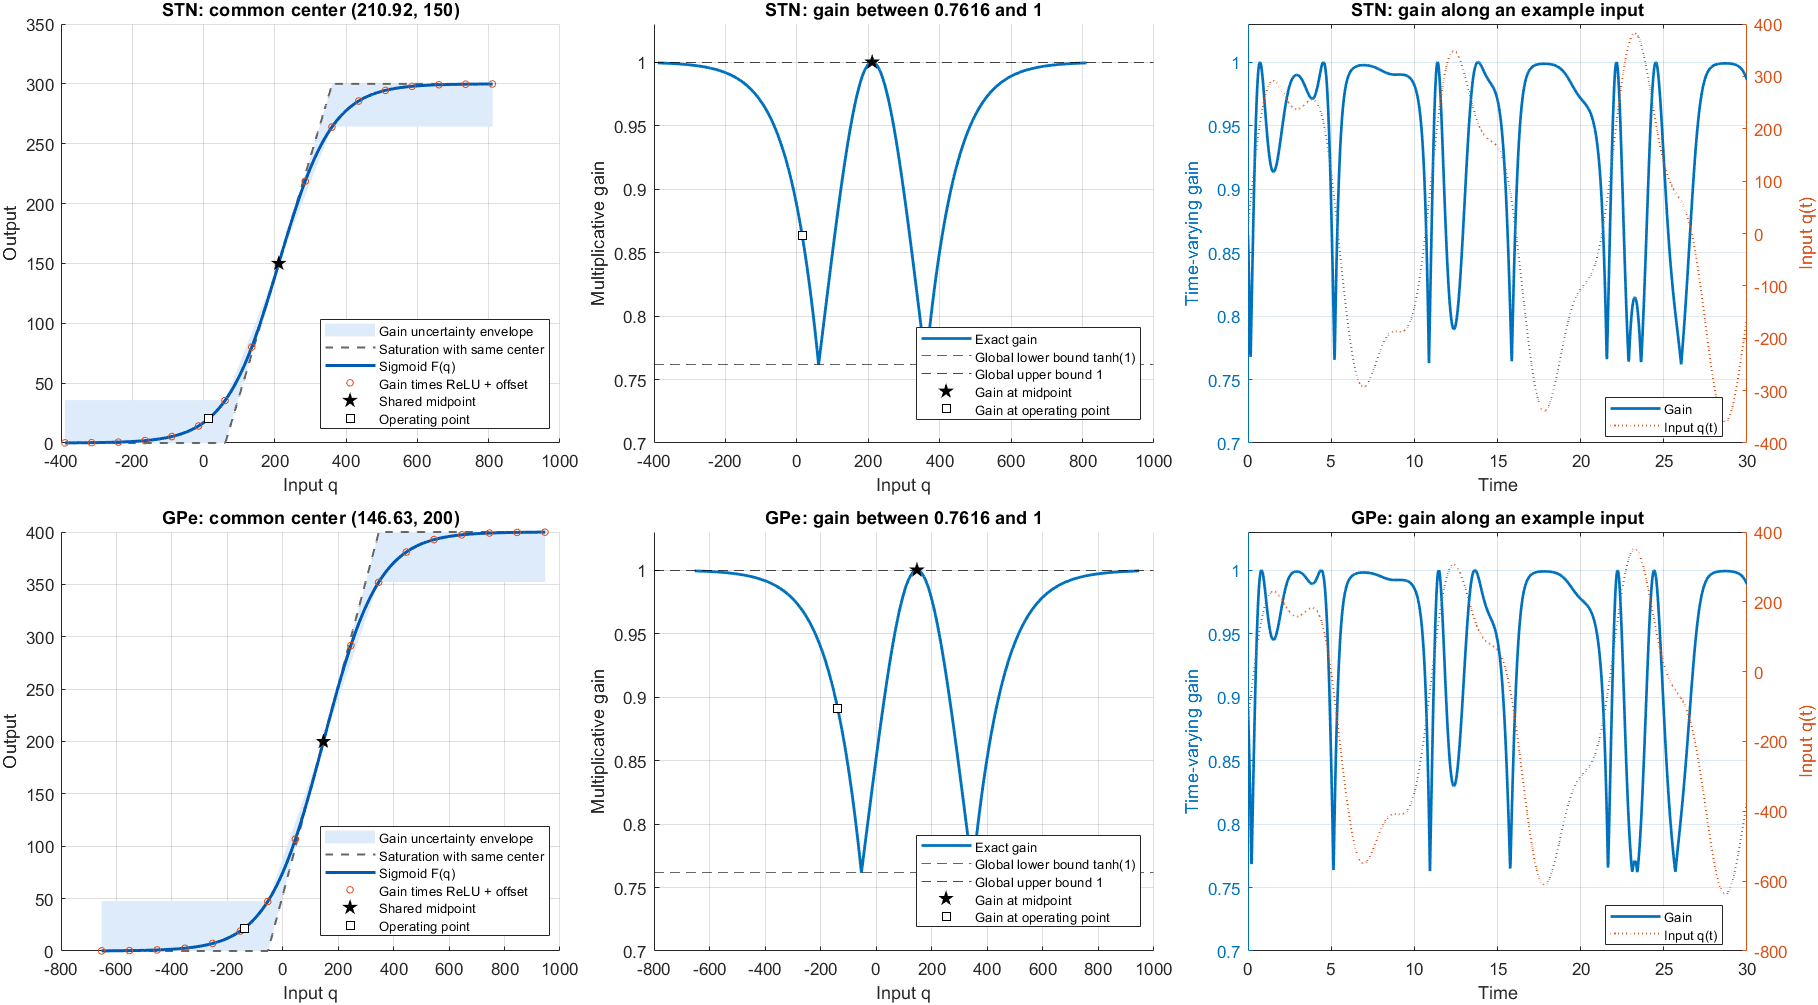
\includegraphics[width=.82\linewidth]{sigmoid_relu_uncertainty.png}\par}
{\small\textcolor{ink}{\textbf{Figure 1.}} The STN (top) and GPe (bottom) examples [4] use \(\ell=0,\ h=M,\ k=1\). The columns show the sigmoid and saturation, the gain \(\theta(q)\), and that gain along one input trajectory.}

\subt{Which gain enters incremental synthesis?}
For two inputs, write \(s_i=\sat_{[-a,a]}(k(q_i-c))\) and \(S(q_i)=b+s_i\). Then \(\Delta F=\theta(q_1)s_1-\theta(q_2)s_2\).
The repeated-scalar multiplier \( [Q,S;-S,-Q] \), with \(Q=Q^\top\succ0\) and \(S=-S^\top\), assumes one shared normalized parameter \( |\delta(t)|\le1 \) on both trajectories.
Allowing independent gains gives a four-vertex box, but its mixed vertices can
produce a nonzero difference even when the inputs coincide.

Use \(\Delta F=\lambda\Delta q\) instead. The secant is the average of
\(F'(q)=k\operatorname{sech}^2(k(q-c)/a)\) between the two inputs. The sharp closed slope bounds are
\[
\begin{aligned}
 0\le\lambda\le k &\qquad\text{globally},\\
 k\operatorname{sech}^2(kL/a)\le\lambda\le k
 &\qquad\text{if both } |q_i-c|\le L,\quad L>0 .
\end{aligned}
\]
For scalar state feedback these give the two endpoint plants of page 3.
Different channels can have different secants.
\vfill
{\footnotesize\color{ink}\textbf{References and project files}\par
[1] Lenssen et al., \emph{Dual Integral Quadratic Constraint Representations for Robust Control of Partial Integral Equations}, Def.~7, route R.2, Cor.~4 (supplied manuscript).\par
[2] Vahedi Noori et al., \href{https://arxiv.org/abs/2407.06888}{\emph{A Complete Set of Quadratic Constraints for Repeated ReLU and Generalizations}}, Thms.~1 and 3 (2024).\par
[3] \texttt{saturation\_iqc.tex} and \texttt{saturation\_iqc\_dual\_synthesis.m}, \texttt{Code/ReLU\_IQC/}.\par
[4] Figure from \texttt{sigmoid\_relu\_uncertainty\_example.m}. Generic form: \texttt{sigmoid\_saturation.m}.}
\newpage\normalsize
\topic{DUAL IQC TYPES}{Plant-side IQCs for ReLU and saturation}
The following are finite-dimensional extensions in the notation of [1, Sec.~VII-F]. Each lemma specifies the uncertainty-channel pair for route R.2. Take a strictly proper uncertainty port (\(D_\Delta=0\)) and a well-posed finite-dimensional plant. The performance channel and remaining R.2 hypotheses are as in [1]. For the dual blocks write
\[
 H=\underline{\mathcal V}_\Delta\{Q,S,R\}:=
 \begin{bmatrix}Q&S\\S^\top&R\end{bmatrix},\qquad
 P_H(L):=[I;L]^\top H[I;L].
\]
In Lemmas 2--6 take \(R=R^\top\prec0\) and \(Q-SR^{-1}S^\top\succ0\). These are the synthesis slice and inertia condition, respectively. Page 6 gives the common factorization. For a convex implementation one may enforce \(P_H(L_0)\succ0\) at one fixed tested slope \(L_0\) to ensure the inertia condition.

\begin{lema}[Dual ReLU IQC]
Let \(w_\Delta=\Phi(z_\Delta)\) componentwise. Choose a symmetric dual block matrix \(H\) of inertia \((m,m)\) with \((H^{-1})_{11}\succ0\). For every sign matrix \(D\) require
\[
 R_D^\top(-J^\top H^{-1}J)R_D\in\COP_m,\qquad R_D=[D;(I+D)/2].
\]
Parameterize the dual IQC by \(\underline\Psi_\Delta=I,\ \underline{\mathcal V}_\Delta=H\). Then R.2(i) holds for the uncertainty channel.
\end{lema}
Equivalently choose a balanced-inertia primal \(M\) with \(M_{22}\prec0\) satisfying the orthant tests, and take \(H=\D(M)\). A fixed such weight gives a convex controller step; the displayed inverse test is nonlinear in a free \(H\).

\begin{lema}[Incremental ReLU on a linear plant port]
Let \(v_i=Kx_i+b\) with common bias \(b\) and \(u_i=\Phi(v_i)\). The incremental plant output is \(z_\Delta=K(x_1-x_2)\). Its uncertainty output is \(w_\Delta=u_1-u_2=\Lambda(t)z_\Delta\), where \(\Lambda(t)\in\operatorname{conv}\{\diag(\nu):\nu\in\{0,1\}^m\}\).
Choose \(H\) under the standing assumptions with \(P_H(\diag(\nu))\succeq0\) at each vertex. Then \((\underline\Psi_\Delta,\underline{\mathcal V}_\Delta)=(I,H)\) satisfies R.2(i) for the uncertainty channel. Page 7 gives the signal maps, the hard IQC and a synthesis example.
\end{lema}

\begin{lema}[Dual saturation IQC]
Let \(w_\Delta=\sat_{[\ell,h]}(z_\Delta)\) be scalar, with \(\ell\le0\le h,\ \ell<h\). Choose scalar \(Q,S,R\) such that
\[
 P_H(1)\ge0,\quad U_\pm^\top H U_\pm\in\COP_2,\qquad
 U_-=\begin{bmatrix}\ell&-1\\\ell&0\end{bmatrix},\quad
 U_+=\begin{bmatrix}h&1\\h&0\end{bmatrix}.
\]
Set \(\underline\Psi_\Delta=I,\ \underline{\mathcal V}_\Delta=H\). Then R.2(i) holds for the uncertainty channel. For arbitrary limits, centering the port at its midpoint gives symmetric limits \([-a,a]\), \(a=(h-\ell)/2\).
\end{lema}

\begin{lema}[Dual incremental saturation IQC]
Let \(z_\Delta=u_1-u_2,\ w_\Delta=\sat(u_1)-\sat(u_2)\) for scalar clipping. Choose \(Q,S,R\) with \(P_H(0),P_H(1)\ge0\). Set \(\underline\Psi_\Delta=I,\ \underline{\mathcal V}_\Delta=H\). Then R.2(i) holds for the uncertainty channel. For the certified command domains on page 3 the restricted test uses \(3/7\) and \(1\).
\end{lema}
\newpage
\topic{DUAL IQC TYPES}{Plant-side IQCs for sigmoids}
\begin{lema}[Dual sigmoid IQC]
Let \(F\) be the sigmoid on page 4. On the centered port take \(z_\Delta=q-c,\ w_\Delta=F(q)-b\). Choose scalar \(Q,S,R\) such that \(P_H(0),P_H(k)\ge0\). Set \(\underline\Psi_\Delta=I,\ \underline{\mathcal V}_\Delta=H\). Then R.2(i) holds for the uncertainty channel. On the multiplicative-gain port \(z_\Delta=S(q)-b,\ w_\Delta=F(q)-b\), use the gain envelope with endpoints \(\tanh(1),1\).
\end{lema}

\begin{lema}[Dual incremental sigmoid IQC]
Let \(z_\Delta=q_1-q_2,\ w_\Delta=F(q_1)-F(q_2)\). Choose scalar \(Q,S,R\) with \(P_H(\alpha),P_H(k)\ge0\), where \(\alpha=0\) globally. Set \(\underline\Psi_\Delta=I,\ \underline{\mathcal V}_\Delta=H\). Then R.2(i) holds for the uncertainty channel. If both inputs remain within \(L>0\) of \(c\), use \(\alpha=k\,\operatorname{sech}^2(kL/a)\) for that domain.
\end{lema}

\subt{Proofs and factorization}
\emph{Graph tests.} Lemma 1 follows from \([z_\Delta;w_\Delta]=R_D|z_\Delta|\) on each orthant [2, Thm.~1]. For Lemma 2 the secant slopes give \(w_\Delta=\Lambda(t)z_\Delta\) as on page 2. For balanced inertia, nonnegativity of \(H\) on the graph of each symmetric \(\Lambda\) is equivalent to nonnegativity of \(M=\D(H)\) on that graph, by the complementary-subspace inertia identity and \(J\,\operatorname{im}[I;\Lambda]=(\operatorname{im}[I;\Lambda])^\perp\). Since \(R\prec0\), vertex testing suffices by concavity. In the scalar lemmas \(M=-H/\det H\) is a positive multiple of \(H\). The saturation tails in Lemma 3 are \(U_\pm[1;t]\), \(t\ge0\); homogeneity gives the two COP tests. The middle branch has slope 1. For Lemmas 4--6 the attainable slope closures are the indicated intervals (pages 3--4). Concavity again gives the endpoint tests.

\emph{Route R.2(i).} For Lemmas 2--6, block inversion gives \(M_{22}=-(Q-SR^{-1}S^\top)^{-1}\prec0\). In Lemma 1 the same sign follows from \(M_{22}=-(H^{-1})_{11}\). Partition \(M=[A,B;B^\top,C]\), put \(X=A-BC^{-1}B^\top\succ0\), and factor
\[
 M=\Theta^\top\diag(X,C)\Theta,\qquad
 \Theta=\begin{bmatrix}I&0\\C^{-1}B^\top&I\end{bmatrix}.
\]
The static factor and \(\Theta_{22}=I\) have bounded causal inverses. The primal graph inequality integrates on every finite horizon. With \(D_\Delta=0\), the uncertainty input-coordinate feedthrough is \(I\). This proves the stated uncertainty-channel conclusions. A regional slope bound applies on its verified domain, or globally to the associated slope-envelope family. \(\square\)

{\small\textbf{Relation to [1, Lemmas 4--6].} The vertex argument uses the gain polytope pointwise, allowing time-varying secants under R.2. A repeated-real weight requires one normalized scalar shared by the channels. Two trajectories generally have different sigmoid factors \(\theta(q_i)\); their incremental port in Lemma 6 uses a single secant.}
\newpage\normalsize
\topic{WORKED EXAMPLE \quad LEMMA 2}{From the linear port to the synthesis inequality}
\textbf{1. Form the difference of the plant equations.} Suppose
\(\dot x_i=Ax_i+B\Phi(Kx_i+b)\) for \(i=1,2\). With \(e=x_1-x_2\), the same \(K,b\) on both trajectories gives the linear plant
\[
 \dot e=Ae+B w_\Delta,\qquad z_\Delta=Ke .
\]
The uncertainty is confined to \(w_\Delta=\Phi(Kx_1+b)-\Phi(Kx_2+b)\).
For component \(j\), use \(\lambda_j(t)=w_{\Delta,j}(t)/z_{\Delta,j}(t)\) when the denominator is nonzero. ReLU is monotone and 1-Lipschitz, so this ratio is in \([0,1]\). At a zero denominator the numerator is zero, so choose \(\lambda_j=0\). Thus \(w_\Delta=\Lambda(t)z_\Delta\). The slopes are used in the proof only. In the saturation lift on page 3 the same subtraction gives \(z_\Delta=[K;K]e\).

\textbf{2. Verify the hard IQC.} Write \(\Lambda=\sum_\nu\mu_\nu V_\nu\) as a convex combination of diagonal vertices. With \(P_H(L)=[I;L]^\top H[I;L]\) and \(R=H_{22}\preceq0\),
\[
 P_H(\Lambda)-\sum_\nu\mu_\nu P_H(V_\nu)
 =-\sum_\nu\mu_\nu(V_\nu-\Lambda)^\top R(V_\nu-\Lambda)\succeq0.
\]
Hence the vertex LMIs imply \(P_H(\Lambda(t))\succeq0\) at every time. For any port signals \(w=\Lambda(t)z\) and every finite \(T\),
\[
 \int_0^T [z;w]^\top H[z;w]\,dt
 =\int_0^T z^\top P_H(\Lambda(t))z\,dt\ \ge0 .
\]
In this diagonal incremental case the transposed slope equals the original slope, so this calculation applies to either slope graph. For the plant-side signed-inverse construction, the primal weight paired with \(H\) is \(M=\D(H)\), as proved on page 6.

\textbf{3. Solve the finite inequalities.} In dual coordinates the plant is
\(\dot\xi=A^\top\xi+K^\top\eta,\ p=B^\top\xi\).
With \(X=X^\top\succ0\) and \(Z=XK^\top\), its strict dissipation inequality is
\[
 \begin{bmatrix}AX+XA^\top&Z\\Z^\top&0\end{bmatrix}
 +G^\top H G\prec0,\qquad
 G=\diag(B^\top,I),\qquad K=Z^\top X^{-1}.
\]
Indeed \(G[\xi;\eta]=[p;\eta]\), and the first term differentiates \(\xi^\top X\xi\). Impose this inequality together with all vertex LMIs. One convex sufficient choice for the inertia conditions is \(R\prec0,\ Q\succ0\). No trajectory or unknown slope appears in this optimization.

\textbf{Scalar check.} Take \(A=-1,\ B=1,\ X=1\) and \(H=[1,1;1,-2]\). The vertex values are \(P_H(0)=P_H(1)=1\); at any slope the supply is \(z^2[1+2\lambda(1-\lambda)]\ge0\). The synthesis matrix is
\(\left[\begin{smallmatrix}-1&Z+1\\Z+1&-2\end{smallmatrix}\right]\).
Choosing \(Z=-1\) makes it negative definite and gives \(K=-1\). Direct substitution in the original difference dynamics yields \(\dot e=-(1+\lambda(t))e\), confirming decay for every admissible slope.
\end{document}
